
\documentclass[10pt,a4paper]{article}
\usepackage[utf8]{inputenc}
\usepackage[english]{babel}
\usepackage{mathtools}
\usepackage{amsfonts}
\usepackage{amssymb}
\usepackage{graphicx}
\usepackage[nottoc]{tocbibind}
\usepackage{hyperref}
\newtheorem{theorem}{Theorem}[section]
\newtheorem{proof}[theorem]{proof}
\author{Stanley}
\title{Proof of Green’s theorem
	Math 131 Multivariate Calculus}
\begin{document}
	\maketitle
\pagenumbering{arabic}
\tableofcontents

\newpage
\section{Introduction}
 Green's theorem is simply a relationship between the macroscopic circulation around the curve C and the sum of all the microscopic circulation that is inside C. If C is a simple closed curve in the plane, then it surrounds some region D (shown in red \ref{closed curve region.png} ) in the plane. D is the “interior” of the curve C \cite{cite2}.
\begin{figure}[h!]
	\centering
	
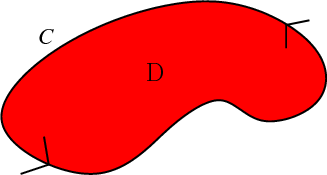
\includegraphics[scale=0.2]{closed_curve_region.png}
\label{closed curve region.png}
\caption{closed curve region}
\end{figure}
Green's theorem says that if you add up all the microscopic circulation inside C (i.e., the microscopic circulation in D), then that total is exactly the same as the macroscopic circulation around C (as shown in \ref{macroscopic_microscopic_circulation.png}).
\begin{figure}[h!]
	\centering
	
	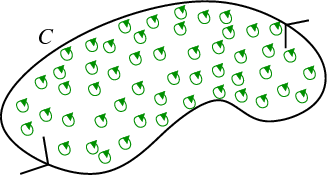
\includegraphics[scale=0.2]{macroscopic_microscopic_circulation.png}
	\label{macroscopic_microscopic_circulation.png}
	\caption{macroscopic-microscopic circulation}
\end{figure} 
\section{Theorem}
 \begin{theorem}[Greens theorem]
 $$\oint_{\delta D}M {dx}+ N {dy}=\iint_{D}\left(\frac{\delta N}{\delta x}-\frac{\delta M}{\delta y}\right) dA$$\label{Green}
 Green’s theorem can be interpreted as a planer
 case of Stokes’ theorem\ref{stoke} \cite{cite2}
 
 $$\oint_{\delta D}{F.}ds=\iint_D\left(\bigtriangledown\times F\right). {k} dA$$\label{stoke}
 In words, that says the integral of the vector field
 F around the boundary $\delta D$ equals the integral of
 the curl of F over the region D. In the next chapter
 we’ll study Stokes’ theorem in 3-space \ref{stoke}.
 Green’s theorem implies the divergence theorem in the plane.
 
It says that the integral around the boundary $\delta D$ of the the normal component of the vector field $F$ equals the double integral over the region D of the divergence of ${F}$ 
\end{theorem}

\begin{proof}
We’ll show whyGreen’s theorem is true for elementary regions D These regions can be patched together to give more general regions \cite{ref1}.

First, suppose that D is a region of  that is, it can be described by inequalities ${a}\leq{x}\geq{b}$ and $\gamma\left(x\right){y}\leq\delta\left(x\right)$ where $\gamma$ and $\delta$ are $C^{1}$ where functions First, we’ll show that	
	
$$\iint_{D}-\frac{\partial M}{\partial y}dA=\oint_{\partial D}M\left(x,y\right)dx$$
We can directly integrate the left integral as a dou-
ble integral
$$\iint_{D}-\frac{\partial M}{\partial y}dA$$

$$=\int_{a}^{b}\int_{\gamma\left(x\right)}^{\partial \left(y\right)} -\frac{\partial M}{\partial y}dydx$$

$$=\int_{a}^{b}-M\left(x,y\right)\lvert_{y=\gamma\left(x\right)}^{\partial\left(x\right)}\quad dx$$
$$\quad\quad=\int_{a}^{b}\left(M\left(x,\gamma\left(x\right)\right)-M\left(x,\partial\left(t\right)\right)\right)dx$$
$$\quad\quad=\int_{a}^{b}M\left(t, \gamma\left(t\right)\right)dt-\int_{a}^{b}\left(t,\delta\left(t\right)\right)dt$$	
We’re almost done. The first integral
$$\int_{b}^{a}M\left(t,\gamma\left(t\right)\right)dt$$\\
is the path integral along $y=\gamma\left(x\right)$ from the left to right, that is, it is $\quad\int_{\gamma} 
M\left(x,y\left(t\right)\right)$ likewize' the second integral $\int_{a}^{b}\left(t,\partial\left(t\right)\right)dt$ is the parameterization along the curve $y=\partial\left(x\right)$ from left to right,but that 
portion of the boundary $\delta D$ should go with from right to left, and the minus sign reverses the 
orientation. The two vertical sides $x=a$ and $x=b$ of D form the other two parts of $\delta$D. since $\frac{dx}{dt}$  on those vertical paths, therefore\\
$$\int M\left(x,y\right)dx=\int M\left(x,y\right)\frac{dx}{dt}dt= \int0dt=0$$
along them. therefore,
$$\int_{a}^{a} M\left(t,\gamma\left(t\right)\right)dt-\int_{a}^{b}\left(t,\partial\left(t\right)\right)dt=\oint_{\delta D}M\left(x,y\right)dx$$\label{type 1}

\end{proof}
 

Likewise, if D is a region of “type 2,” that is, one bounded between horizontal lines, then\\
$$\iint_{D}\frac{\partial D}{\partial N} dA=\oint_{\delta D} N\left(x,y\right)dy$$\label{type 2}
where the minus sign is dropped because the symmetry exchanging y for x reverses orientation.Adding these two equations \ref{type 1} and \ref{type 2} gives Green’s theorem for D
$$\iint_{D}\left(\frac{\partial N}{\partial x}-\frac{\partial M}{\partial y}\right)dA=\oint_{\partial D}M\left(x,y\right)dx+ N\left(x,y\right)dy$$
That takes care of the case when the region is of
both type 1 and type 2. But regions that can be
decomposed into a finite number of these can be
patched together to take care of the general case.
q.e.d.\cite{ref1}
There are other proofs that are more inclusive
to show that some regions that are a union of an
infinite number of these regions also satisfy Green’s 
theorem.

\bibliographystyle{unsrt}
\bibliography{stanley_akor_ICL1}


	\end{document}